\documentclass[oneside, abstracton, titlepage]{scrartcl}

\usepackage[left=2.5cm,right=2.6cm,top=3cm,bottom=3cm]{geometry}
\usepackage[utf8]{inputenc}
\usepackage[intlimits]{amsmath}
\usepackage{amssymb}
\usepackage{color}
\usepackage{subcaption}

\usepackage{graphicx}

\begin{document}
	\title{Discovering governing reactions from concentration data}
	\maketitle
	
	\section{Introduction}
	When presented with a non-equilibrium time series of possibly noisy concentration fluctuations of some species as output of, e.g., measurements from experiments or simulations that were parameterized by microscopic rates \textcolor{red}{(cite ReaDDy?)}, one can ask for the corresponding macroscopic rates and generating reaction network. 
	In this paper we present an application of the shallow learning method SINDy \cite{Brunton2015}. It is able to identify the generating parsimonious nonlinear dynamics in data that stems from dynamical systems, thus providing an interpretable result.
	In our application we, opposed to the original method, do not only look for macroscopic rates of net species change but investigate the specific reactions that might have lead to the observations.
	We demonstrate the algorithm on two toy problems - one problem showing that when there is no ambiguity in the system, one converges to the correct rates with increasing resolution of concentration fluctuations and one in which we compute a sparse reaction network for given data.
	
	\section{The method}
	The underlying model that we want to fit the data to is a law of mass action type dynamical system. To this end, let $S$ be the number of species, then the concentration data at a time $t$ can be represented by a vector
	\begin{align}
	\mathbf{x}(t)=\begin{pmatrix}
	x_1(t)\\ \vdots \\ x_S(t)
	\end{pmatrix}\in \mathbb{R}^S.
	\end{align}
	Further, one can choose $R$ possible ansatz reactions with their respective reaction function
	\begin{align}
	\textbf{y}_r(\textbf{x}(t))=\begin{pmatrix}
	y_{r,1}(\textbf{x}(t)) \\ \vdots \\ y_{r,S}(\textbf{x}(t))
	\end{pmatrix}
	\end{align}
	so that the change of concentration for species $i$ at time $t_i$, is represented by the dynamical system
	\begin{align}
	\dot{\textbf{x}}_i(t) = \sum_{r=1}^{R}y_{r,i}(\textbf{x}(t))\xi_r,\quad i=1,\ldots, S,
	\label{method:the-system}\end{align}
	where $\xi_r$ are the to-be estimated macroscopic rates.
	
	When presented with a time series with $T$ observations, the data can be represented as a matrix
	\begin{align}
	\textbf{X} = \begin{pmatrix}
		x_1(t_1) & x_2(t_1) & \cdots & x_S(t_1) \\
		x_1(t_2) & x_2(t_2) & \cdots & x_S(t_2) \\
		\vdots   & \vdots   & \ddots & \vdots   \\
		x_1(t_T) & x_2(t_T) & \cdots & x_S(t_T)
	\end{pmatrix} \in \mathbb{R}^{T\times S}.
	\end{align}
	Given this matrix, one can propose a library $\Theta(\textbf{X}) = \begin{pmatrix} \theta_1(\textbf{X}) & \theta_2(\textbf{X}) & \cdots & \theta_R(\textbf{X}) \end{pmatrix}$ of $R$ ansatz reactions with corresponding reaction functions
	\begin{align}
		\theta_r(\textbf{X}) = \begin{pmatrix}
		\textbf{y}_r(\textbf{X}_1)^T \\ \vdots \\ \textbf{y}_r(\textbf{X}_T)^T
		\end{pmatrix}\in \mathbb{R}^{T\times S},\quad r=1,\ldots,R,
	\label{method:the-reactions}\end{align}
	where $\textbf{X}_i$ denotes the $i$-th row in $X$. Applying the concentration trajectory to the library yields a data tensor $\Theta(\textbf{X})\in\mathbb{R}^{T\times S\times R}$. Following the approach of SINDy, the goal is now to find coefficients $\Xi = \begin{pmatrix} \xi_1 & \xi_2 & \cdots & \xi_R
	\end{pmatrix}^T$, so that
	\begin{align}
	\dot{\textbf{X}} = \Theta(\textbf{X})\Xi = \sum_{r=1}^{R}\theta_r(\textbf{X})\xi_r.
	\end{align}
	In particular, the system is linear in the coefficients $\Xi$, which makes sparse regression tools such as LASSO \cite{Tibshirani1996, Hastie2009} applicable. To this end, one can consider the minimization problem to find $\hat{\Xi}$ such that
	\begin{align}
		\hat{\Xi} = \underset{\Xi}{\arg\min}\left( \frac{1}{2T}\left\| \dot{\textbf{X}} - \Theta(\textbf{X})\Xi \right\|_F^2 + \alpha\|\Xi\|_1 \right) \quad \text{subject to }\Xi \geq 0,
	\label{method:minimizationproblem}\end{align}
	where $\alpha\geq 0$ is a sparsity inducing hyperparameter and $\|\cdot\|_F$ denotes the Frobenius norm. For $\alpha=0$ this problem reduces to constrained least-squares. For solving (\ref{method:minimizationproblem}) we apply the sequential least squares minimizer SLSQP, originally described in \cite{Kraft1988}, contained in, e.g., the software package SciPy \cite{SciPy}. As initial guess for the regulated problem we use the solution of (\ref{method:minimizationproblem}) with $\alpha=0$.
	
	\section{Examples}
	
	\begin{figure}
		\begin{center}
			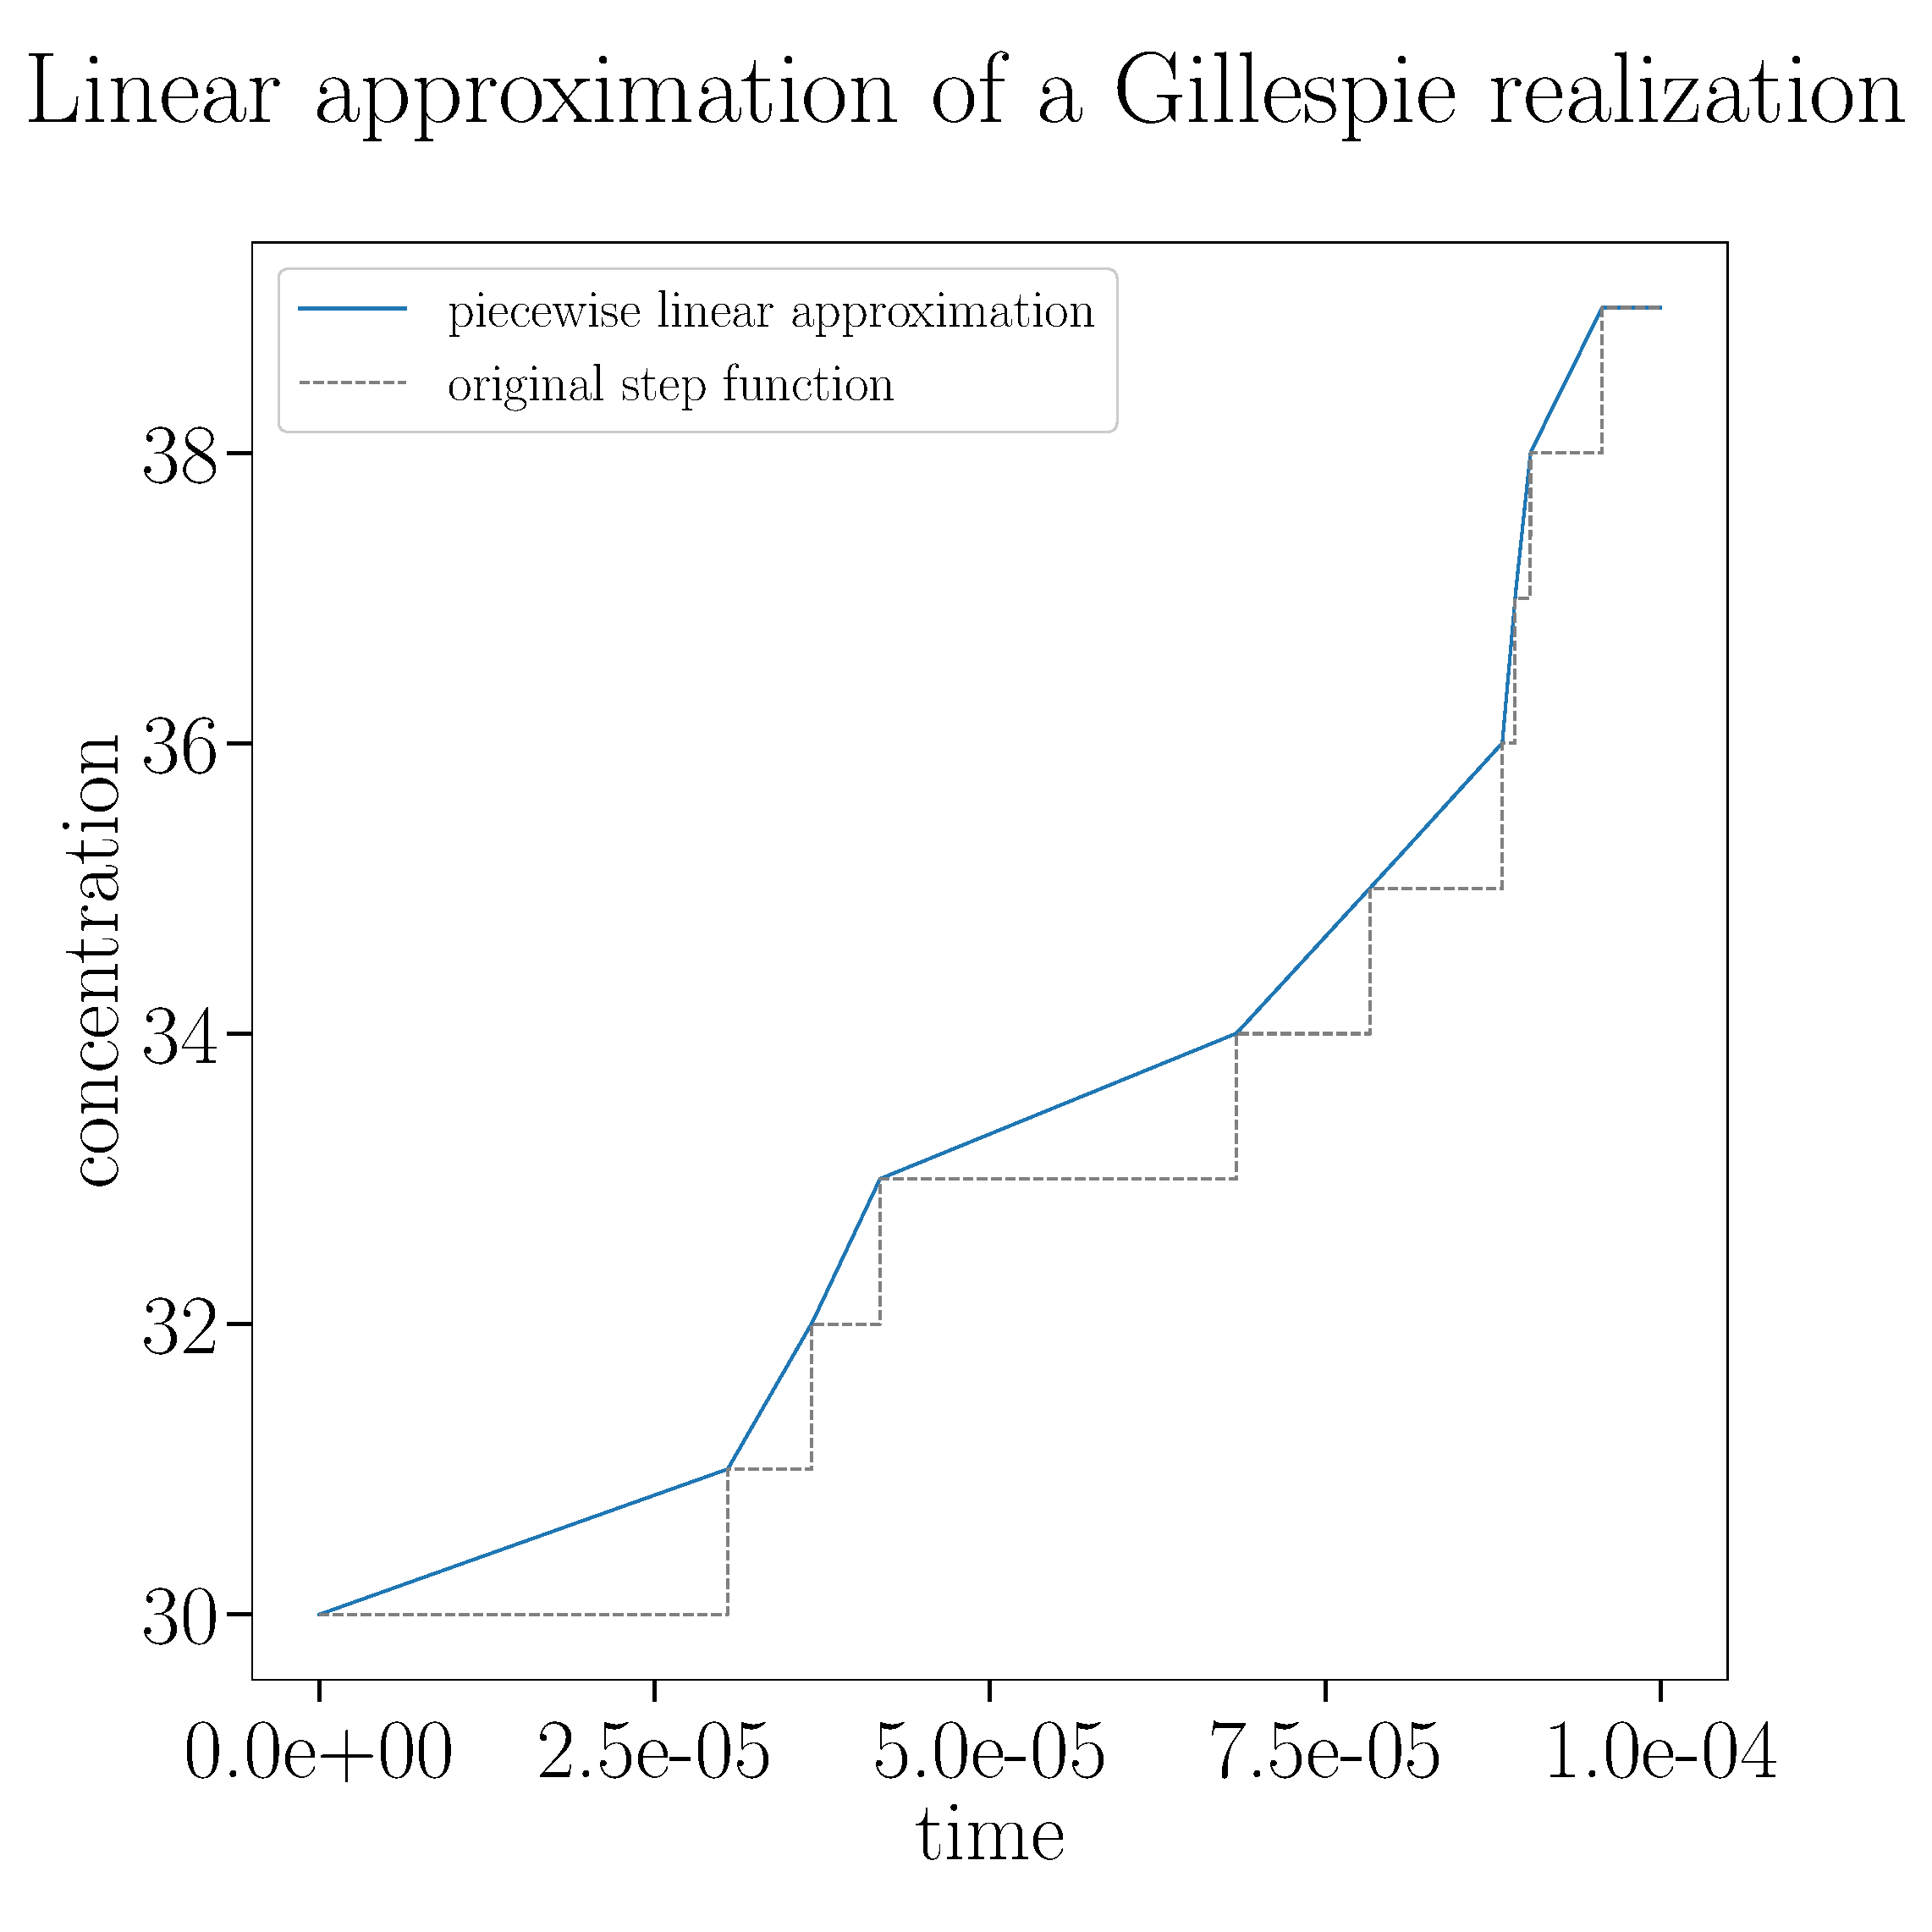
\includegraphics[width=.5\textwidth]{./figures_tex/aux_linear_approximation.eps}
		\end{center}
		\caption{This figure depicts a possible output yielded by an application of the Gillespie method and the performed piecewise linear approximation in order to obtain a better behaving derivative.}
		\label{examples:linear-approximation}
	\end{figure}
	
	For generating time series data of concentrations we use the Gillespie method \cite{Gillespie1976}. For a given set of initial conditions, we produce several realizations which then are converted to a trajectory with fixed time step and averaged. Since these trajectories are piecewise constant, one has to take special care when approximating the temporal derivative. Simply taking finite differences has the effect that, with decreasing time step, the derivative is most of the time constant zero and approaches infinity at the jump discontinuities. To counter this effect, we beforehand perform a linear approximation between each two adjacent discontinuities, as depicted in Figure \ref{examples:linear-approximation}. (\textcolor{red}{Use regularized derivative?})
	
	\subsection{Regression without regularization}
	\label{sec:ex1}
	
	Here we demonstrate that, with decreasing time step $\Delta t$ and $\alpha=0$, the estimated rates converge to the true rates if there is no ambiguity in the system. The systems contains two species $A$ and $B$ which can convert into each other with macroscopic rates of $r_1=4.0$ and $r_2=0.5$, respectively. The initial amount of particles is set to $70$ of type $A$ and $0$ of type $B$. A possibly resulting change of concentrations over time is depicted in Figure \ref{ex1:concentration-curves}.
	
	\begin{figure}
		\begin{center}
			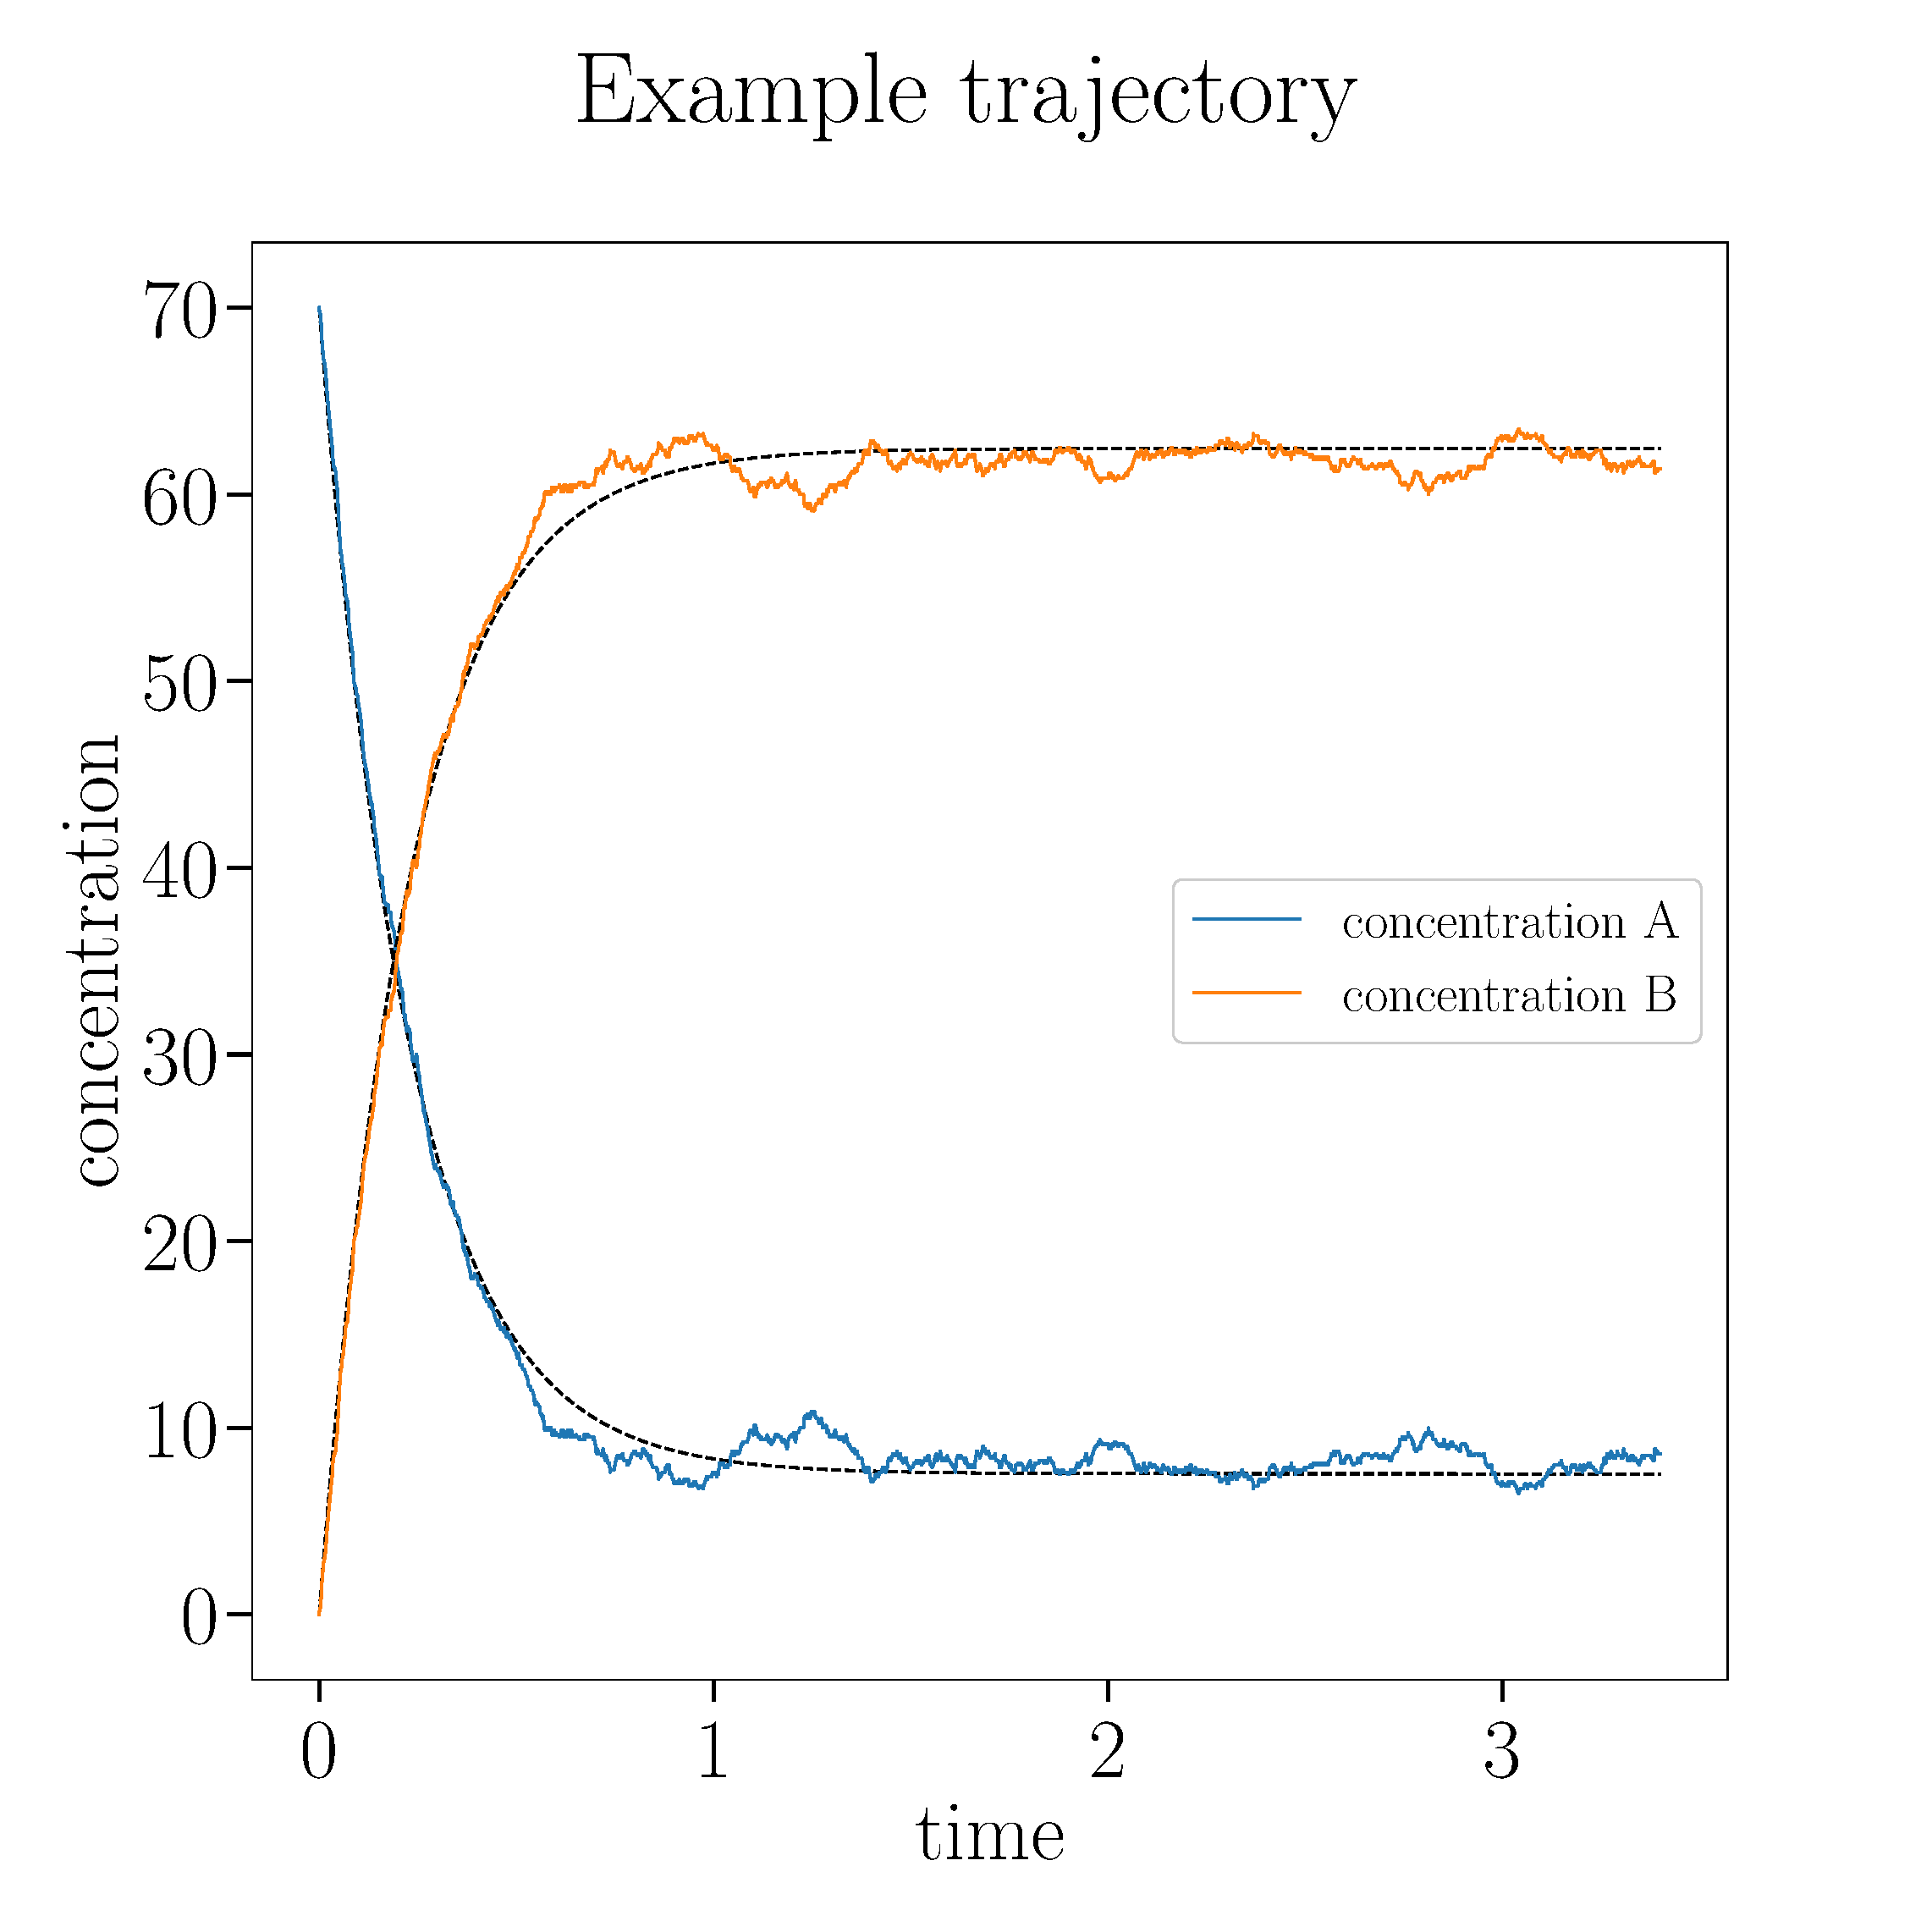
\includegraphics[width=.5\textwidth]{./figures_tex/aux_ex1_concentration_curves}
		\end{center}
		\caption{A realization of the example given in Section \ref{sec:ex1}.}
		\label{ex1:concentration-curves}
	\end{figure}
	
	For each $\Delta t$, we averaged eight different realizations with identical starting conditions into one single trajectory and estimated the rates for reactions $A\to B$ and $B\to A$. This procedure, we repeated $30$ times. In Figure \ref{ex1:rates-convergence}, the average estimates alongside with their standard deviations are shown. One can see that, with decreasing $\Delta t$, also the estimate for the rates becomes better and they can be recovered.
	
	\begin{figure}
		\begin{center}
			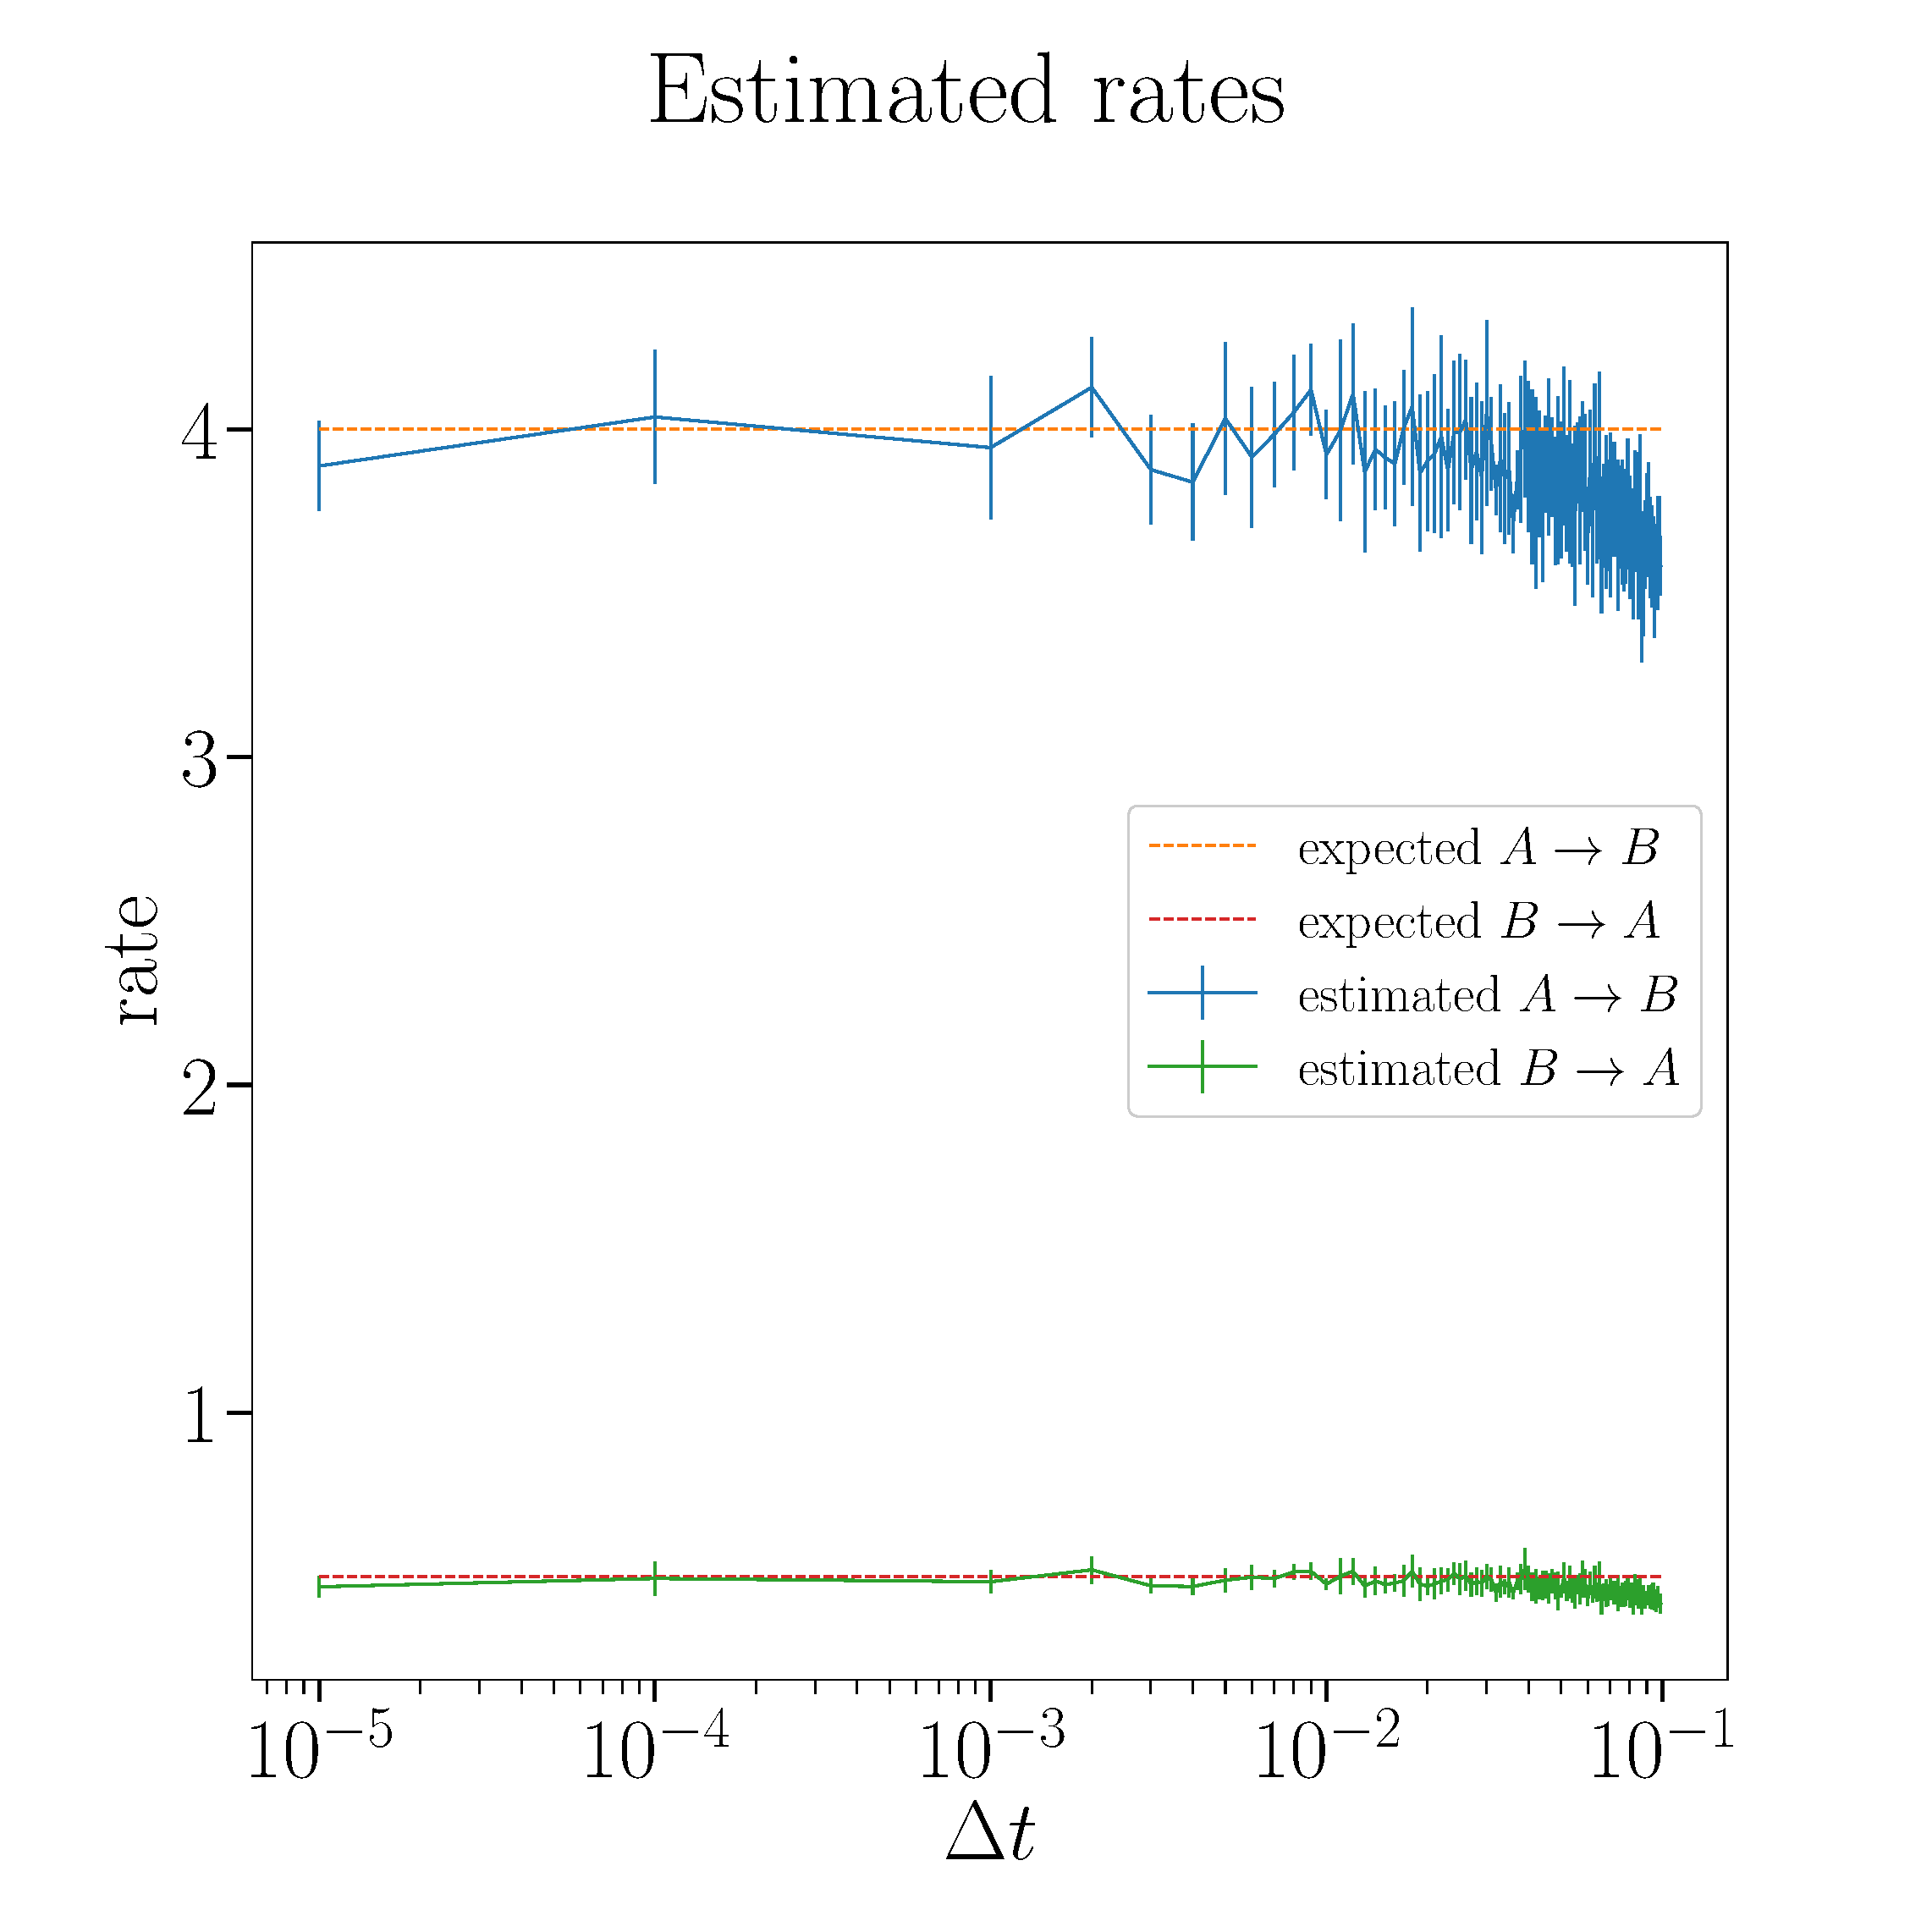
\includegraphics[width=.5\textwidth]{./figures_tex/aux_rates_convergence}
		\end{center}
		\caption{Convergence of estimated rates to the ground truth with decreasing $\Delta t$.}
		\label{ex1:rates-convergence}
	\end{figure}
	
	\subsection{Regression with regularization}
	\label{sec:ex2}
	In this example there are four species $A$, $B$, $C$, and $D$ with reactions $A\xrightarrow{k_1}D$, $D\xrightarrow{k_2}A$, $D\xrightarrow{k_3}B$, $A+B\xrightarrow{k_4}C$, and $C\xrightarrow{k_5}D+B$, where $k_1=k_2=2\cdot 10^{-2}$, $k_3 = 1\cdot 10^{-2}$, and $k_4=k_5=1\cdot 10^{-4}$. These reactions are inserted into the ansatz library $\Theta (\cdot)$. Additionally the reactions $A\leftrightarrow B$, $A\leftrightarrow C$, and $A+C\leftrightarrow D$ are inserted into the library. 
	
	\begin{figure}
		\centering
		\begin{subfigure}[b]{.45\textwidth}
			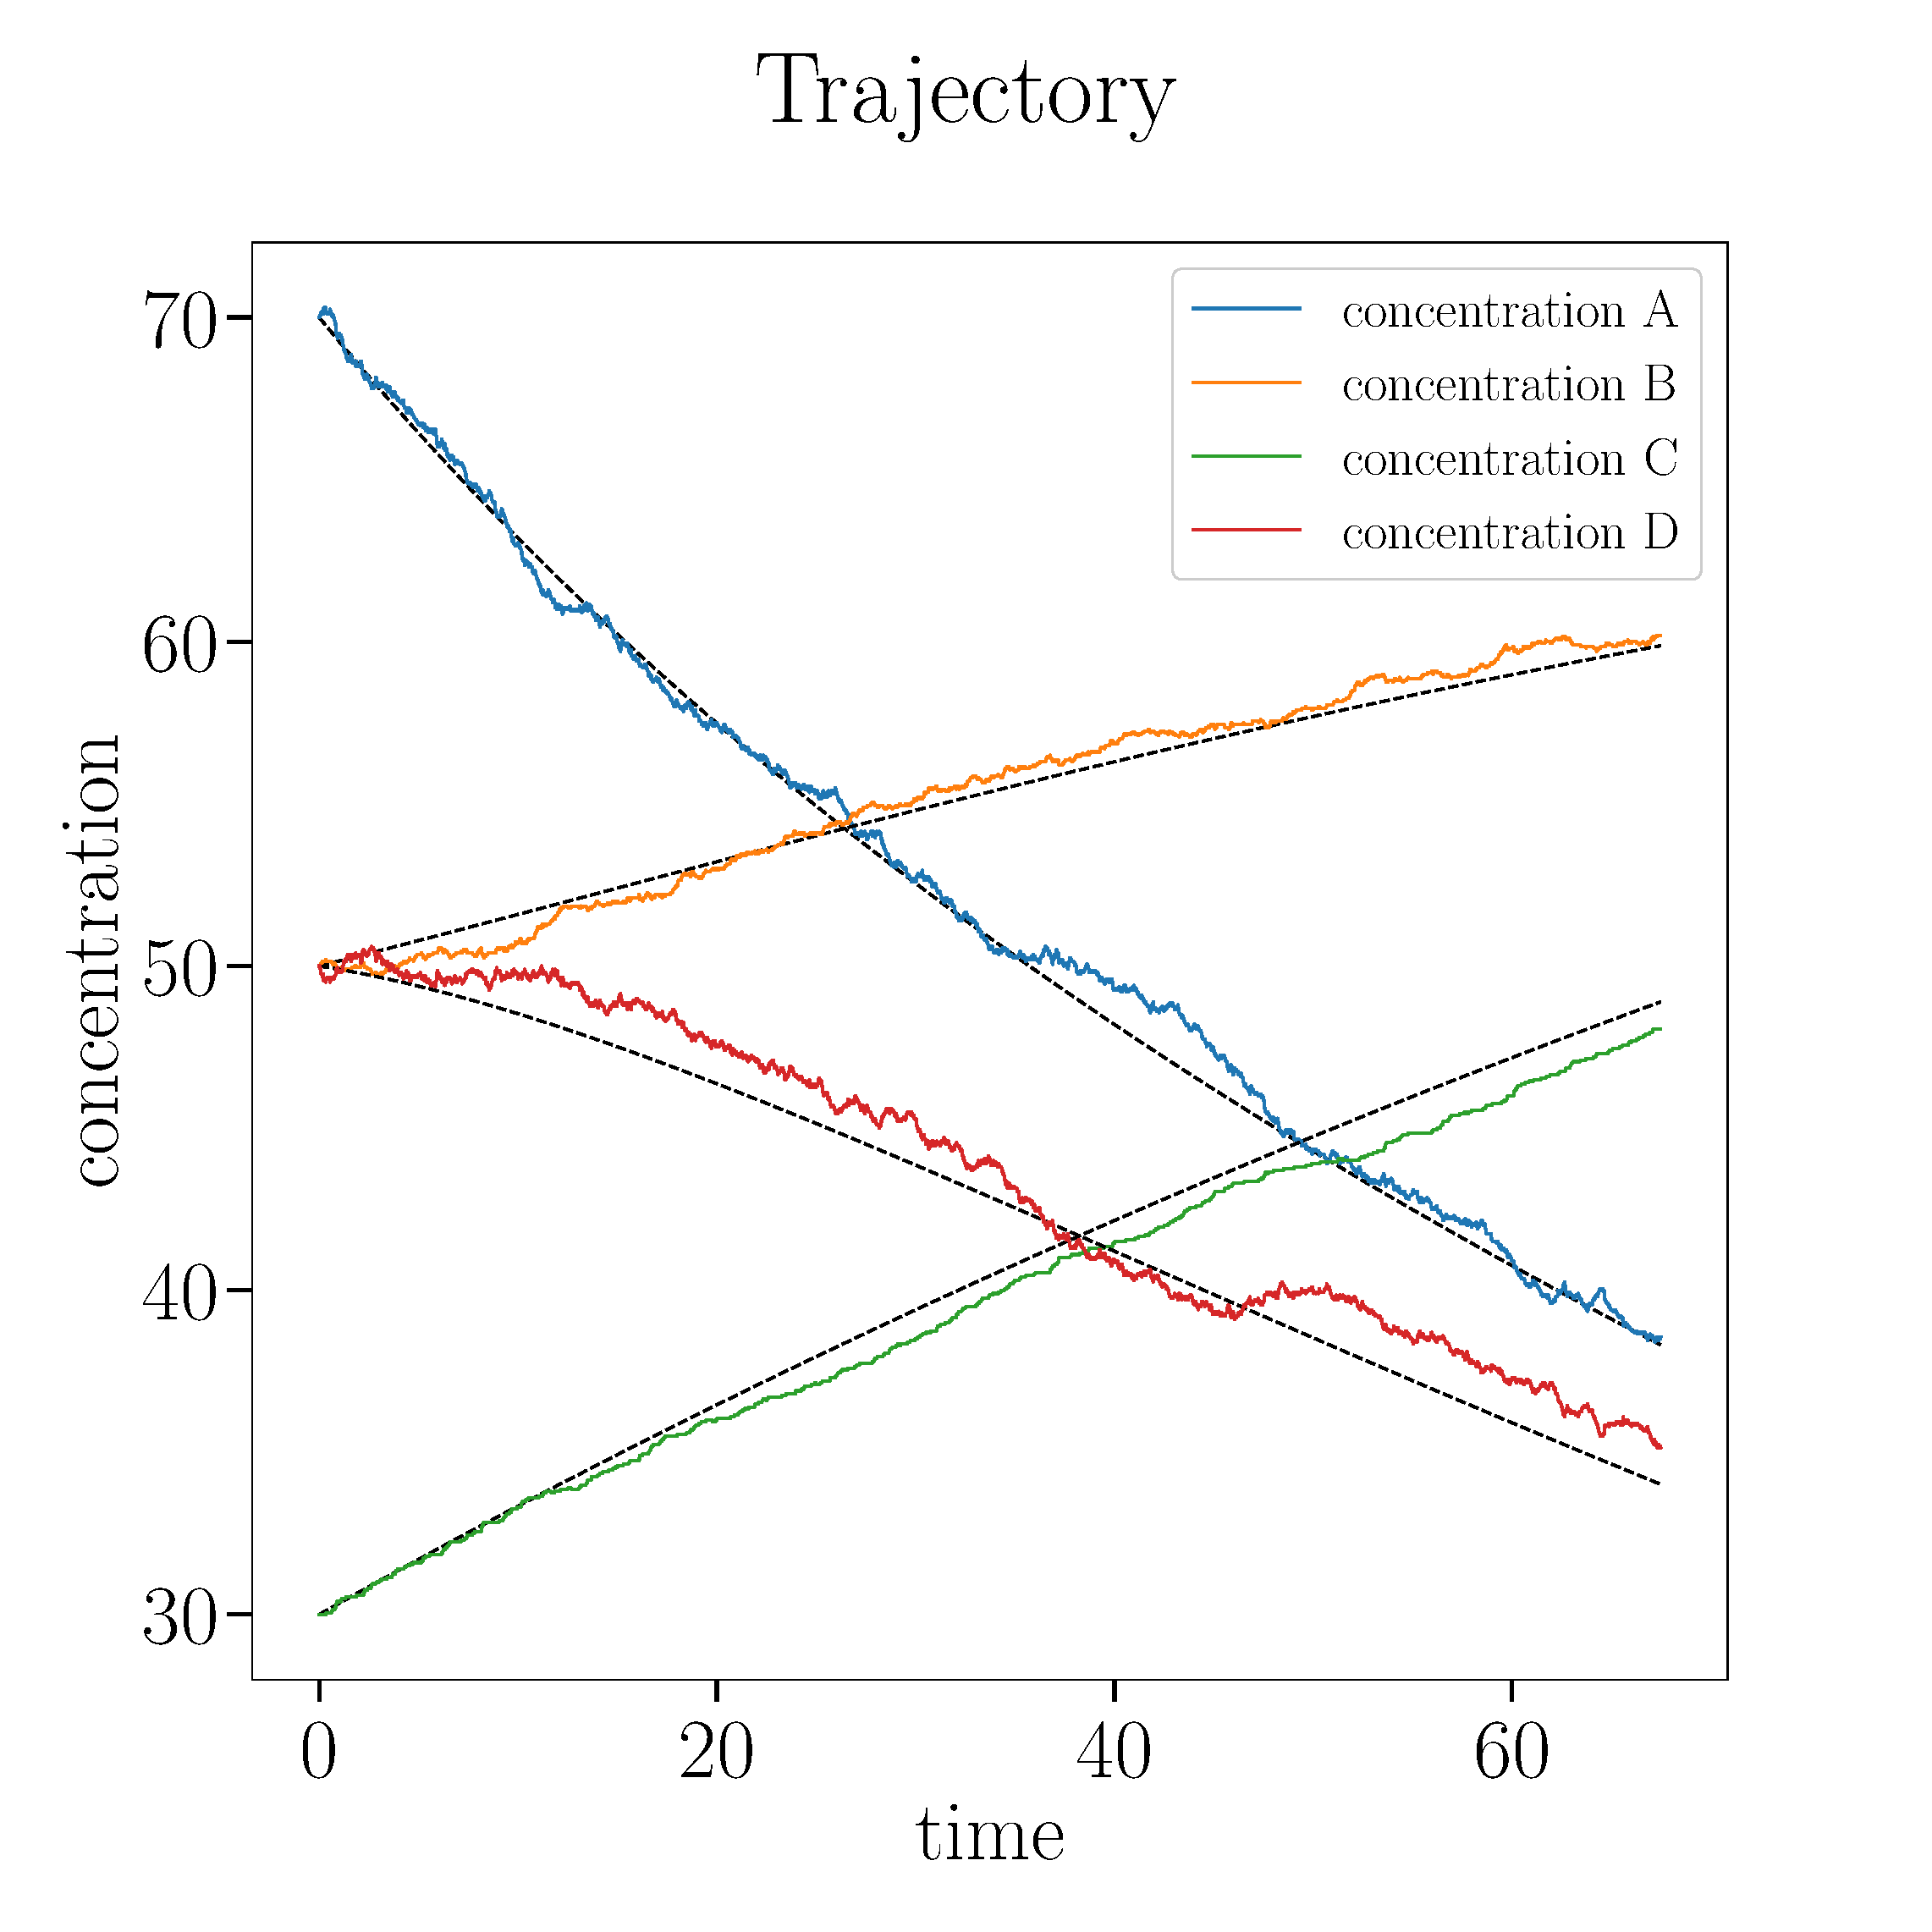
\includegraphics[width=\textwidth]{./figures_tex/cv_concentrations_train}
			\caption{Train data set.}
		\end{subfigure}
		~
		\begin{subfigure}[b]{.45\textwidth}
			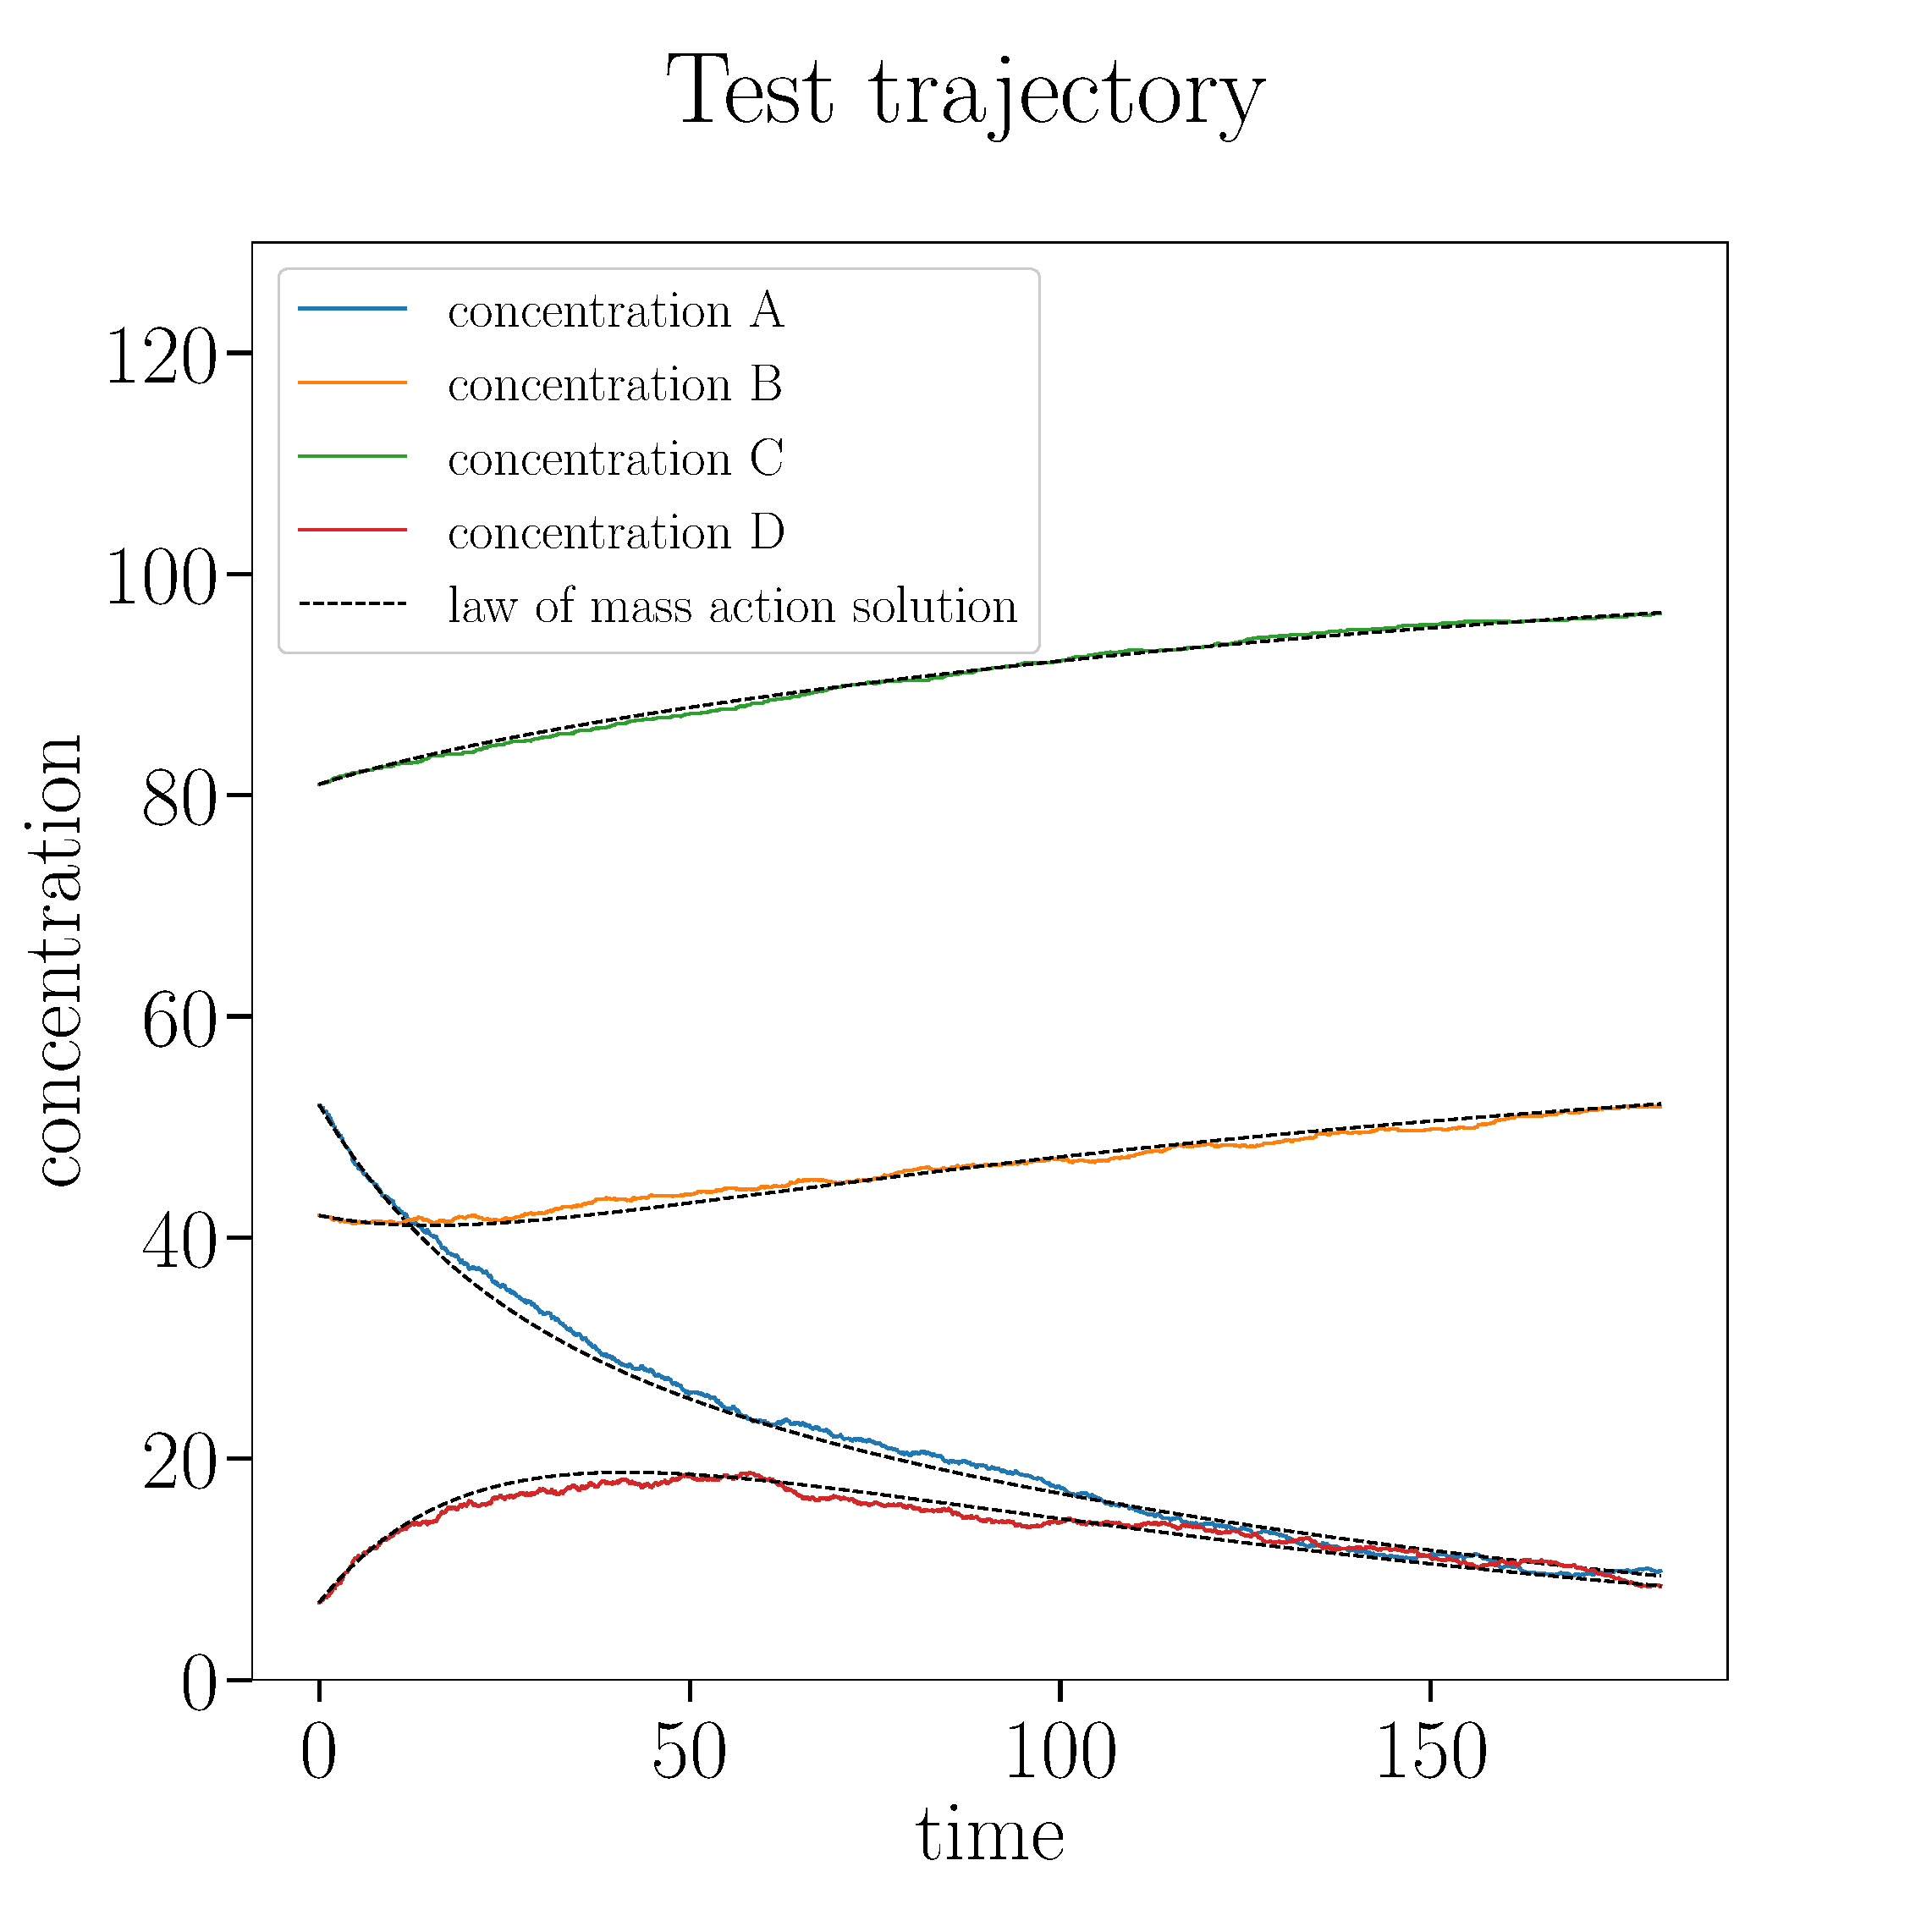
\includegraphics[width=\textwidth]{./figures_tex/cv_concentrations_test}
			\caption{Test data set.}
		\end{subfigure}
		\caption{Train and test data sets for the example given in Section \ref{sec:ex2}.}
		\label{ex2:test-train-concentration-curves}
	\end{figure}
	
	The problem now is to find a suitable $\alpha$ such that a parsimonious solution is picked. To this end, cross-validation is applied. The trajectories that were used as training and test data set are depicted in Figure \ref{ex2:test-train-concentration-curves}. \textcolor{red}{Perhaps use several test trajectories with different initial conditions to get something like a confidence interval?} As an indicator to the estimation error we use the scoring function
	\begin{align}
		f_\alpha = \frac{1}{T}\|\mathbf{\dot{X}}_\text{test} - \Theta (\textbf{X}_\text{test}) \Xi_\text{train}\|_F^2.
		\label{ex2:score-function}
	\end{align}
	For a selection of values $\alpha\in [0, 100]$, the model parameters $\Xi$ were estimated and the scoring function (\ref{ex2:score-function}) evaluated, yielding the graph that is depicted in Figure \ref{ex2:score-graph}.
	
	\begin{figure}
		\begin{center}
			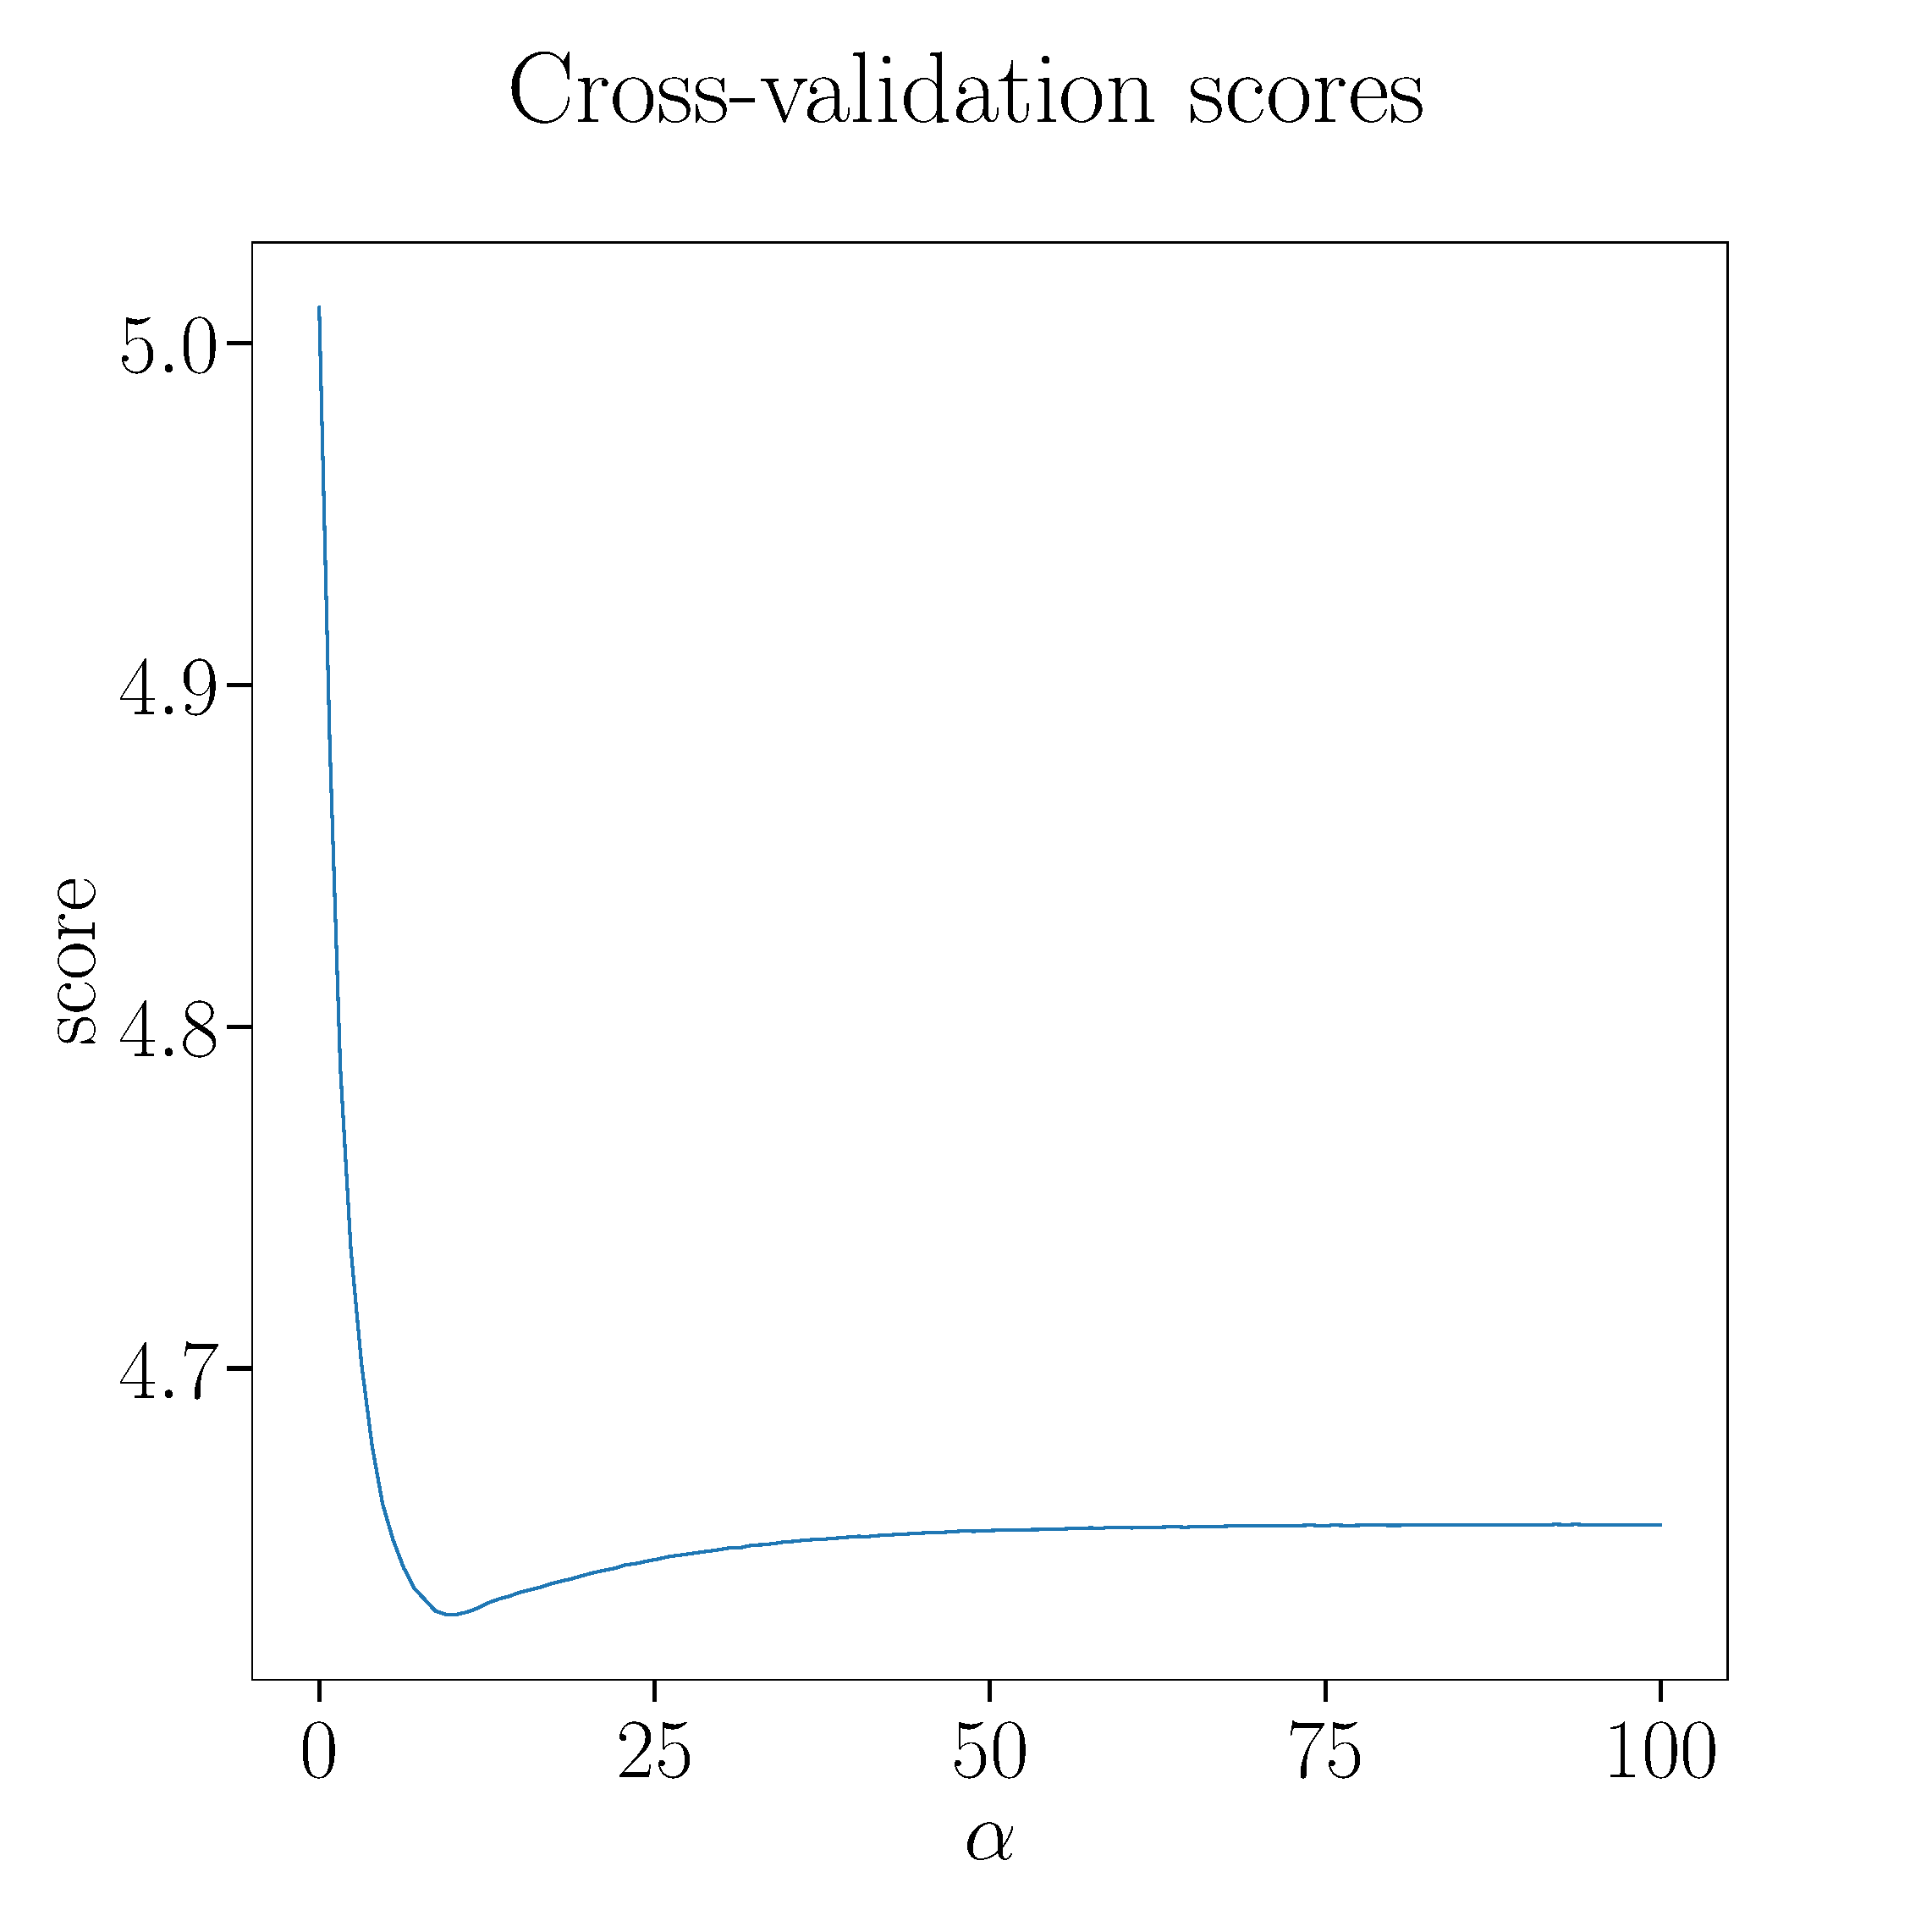
\includegraphics[width=.5\textwidth]{./figures_tex/cv_score}
		\end{center}
		\caption{Score function (\ref{ex2:score-function}) evaluated for a range of $\alpha$ values.}
		\label{ex2:score-graph}
	\end{figure}

	One can see that the minimum is at about
	\begin{align}
		\hat{\alpha} = \underset{\alpha\in[0,100]}{\arg\min}f_\alpha\approx 10.
	\end{align}
	When evaluating the minimization problem (\ref{method:minimizationproblem}) with $\hat{\alpha}$ as hyperparameter for the regularizer and applying a cut-off of $10^{-10}$ to the yielded parameters, one obtains the simpler set of reactions $A\xrightarrow{\hat{k}_1}D$, $D\xrightarrow{\hat{k}_3} B$, and $A+B\xrightarrow{\hat{k}_4}C$ with rates $\hat{k}_1 \approx 3.5\cdot 10^{-3}$, $\hat{k}_3\approx 9.1\cdot 10^{-3}$, and $\hat{k}_4\approx 8.7\cdot 10^{-5}$, respectively.
	
	One can see in Figure \ref{ex2:result} that with this simpler set of reactions the observed concentration curves can be explained as well. It can be argued that the second reaction of the generating model $D\xrightarrow{k_2}A$ can be compensated by a smaller rate $\hat{k}_1 < k_1$ and that the fifth reaction of the generating model can be neglected altogether in the observed timescale as its rate is two orders of magnitude smaller than the rates of the other unimolecular reactions. 
	The rates $k_3$ and $k_4$ are approximately recovered by $\hat{k}_3$ and $\hat{k}_4$, respectively.
	
	\begin{figure}
		\begin{center}
			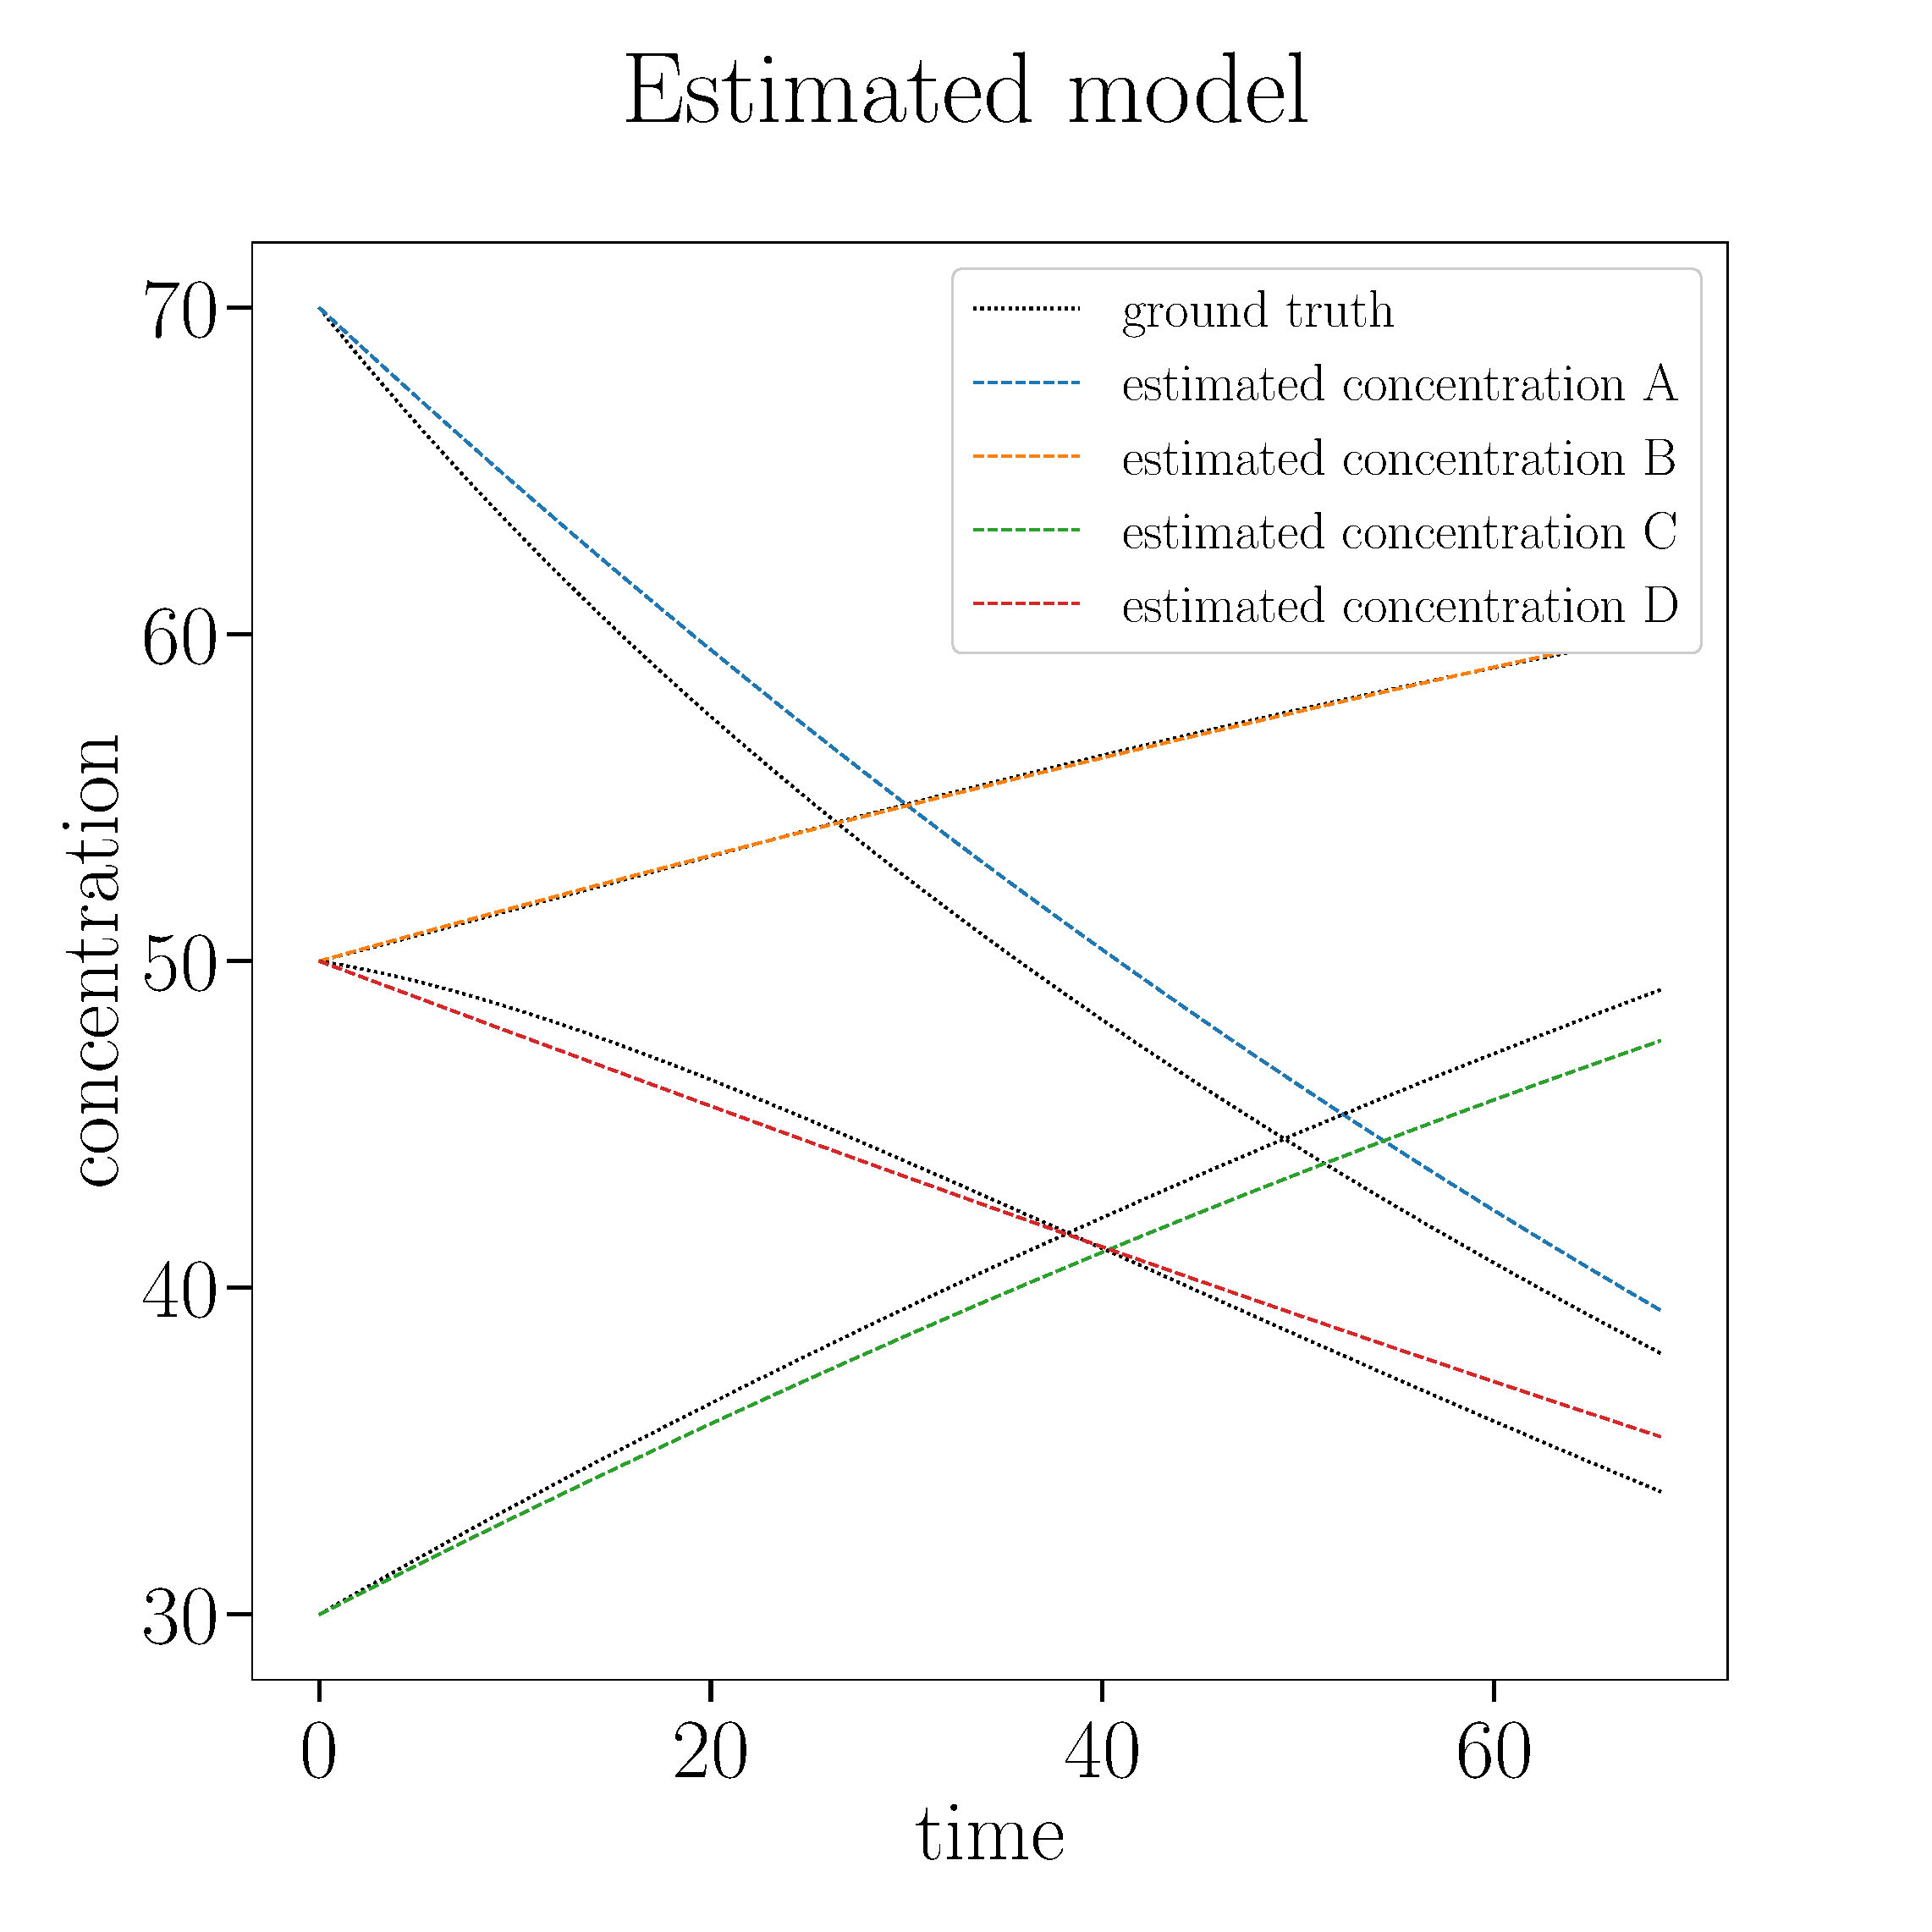
\includegraphics[width=.5\textwidth]{./figures_tex/cv_expected_estimated_concentrations}
		\end{center}
		\caption{Estimated and generating concentration curves for the example in Section \ref{sec:ex2}.}
		\label{ex2:result}
	\end{figure}
	
	\section{Conclusion}
	In this work we have successfully applied and extended the SINDy method to not only parsimoniously detect potentially nonlinear terms in a dynamical system from possibly noisy data, but also pick up on, in this case, a sparse set of generating reactions (\ref{method:the-reactions}) and their respective rates.
	
	In two examples it was demonstrated that, despite noisy data and unavailability of derivative measurements, a parsimonious generating reaction network that is able to explain the observed data can be recovered. 
	In particular it was shown in the example given in Section \ref{sec:ex1} that if there is no ambiguity in the underlying model and ansatz reaction library, the actual rates can be recovered. In the example of Section \ref{sec:ex2} an even simpler model could be obtained by making use of sparse regression and cross-validation.
	
	\newpage
% 	\bibliographystyle{alpha}
	\bibliographystyle{abbrv}
	\bibliography{bibliography.bib}
	
\end{document}
